\documentclass[12pt,a4paper]{report}
\usepackage[utf8]{inputenc}
\usepackage{multicol,caption}
\usepackage{amsmath}
\usepackage{amsfonts}
\usepackage{amssymb}
\usepackage[left=2cm,right=2cm,top=2cm,bottom=2cm]{geometry}
\title{\huge {\textbf{Image Stritching}}}
\author{\LARGE \centerline{
Authors: Yehuda Neumann, Yakir Arie, Mark Gurin}
\\* 
\\* {IDs:  305539066, 205387491, 320755499 }
\\*{Department of Computer Science
}
\\ {Computer Vision and Image Processing}
\\*
{Ariel University}
\\*
\\* {Advisor: Dr. Gil Ben-Artzi}}
\date{\centerline {October, 2019}}
\usepackage{natbib}
\usepackage{graphicx}
\graphicspath{ {./images/} }


\begin{document}
\maketitle
\section*{Introduction To Image Stitching}
The problem:
From series of photos that were made from static rotating camera, we have to  create one image that will represent the space, where the original made images transformed to the other image’s plane. To achieve that task a couple of setting should be done.
before diving into the result and the process let's figure out what are the difficulties that we will have to deal with.
Stitching errors are a common problem in panoramic photography, where the photo stitching software made a mistake in lining up the images when it stitched them together. After stitching your panorama you might see some places where objects have been distorted, misaligned or cut in half during the panorama stitching process, like in this example:

\begin{figure}[h]
\centering
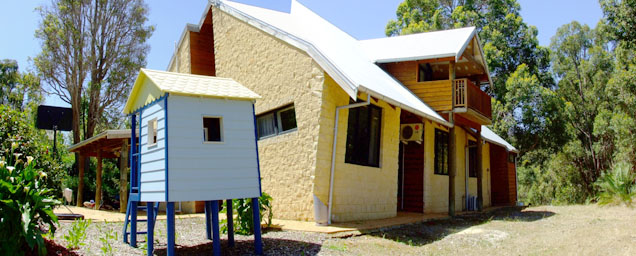
\includegraphics[width=8cm]{p4-stitch-error}
\captionof{figure}[6.5pt]{Panorama stitching errors caused by distortion and lack of overlap.}
\end{figure}

\begin{figure}[h]
\centering
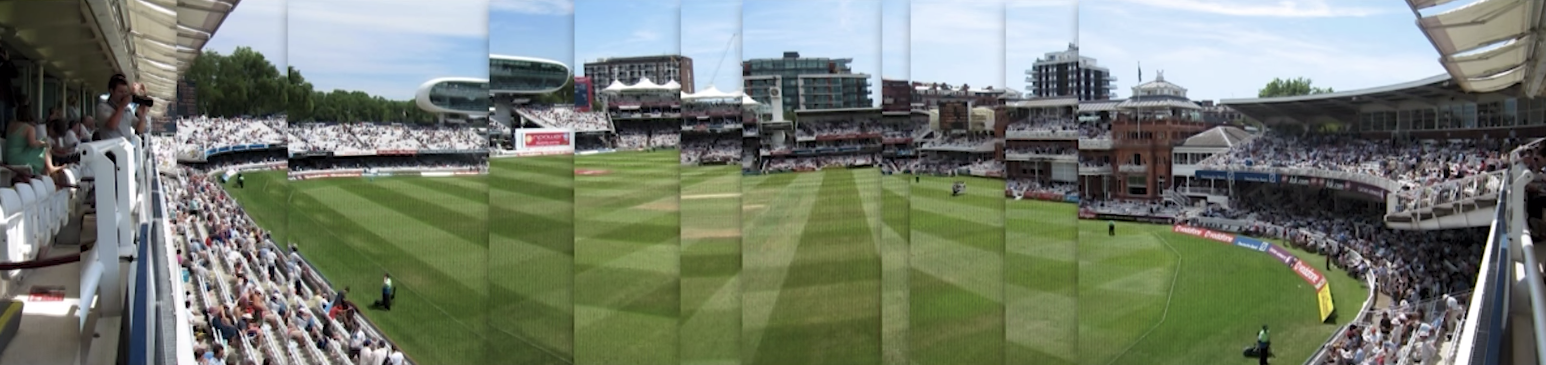
\includegraphics[width=8cm]{seriesofphotos}
\captionof{figure}[6.5pt]{Series of photos  }
\end{figure}

\begin{figure}[h]
\centering
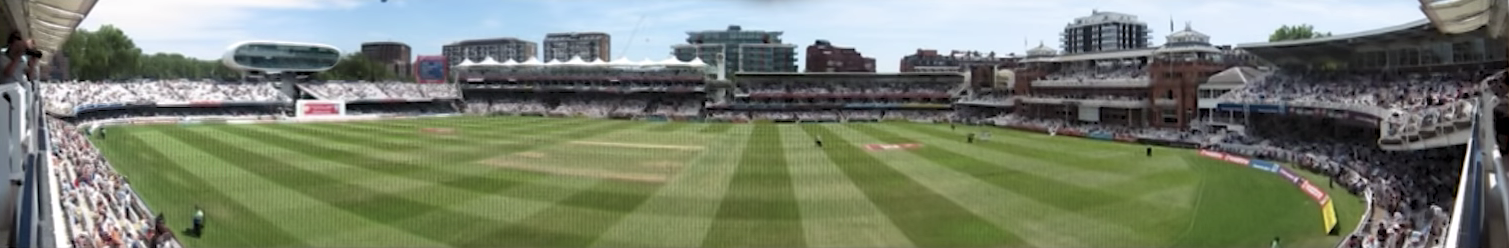
\includegraphics[width=8cm]{panoramfinal}
\captionof{figure}[6.5pt]{Final result of panorama}
\end{figure}

\section*{Approach and Method}
The main problem is to find the best Homography matrix that will move each pixel to the right place s.t the set of images will looks like one complete image without distortions.
to find the Homography and achieve image stitching we have to follow the basic steps:
\begin{itemize}
	\item  Detect keypoints in each  image
	\item  Match the most common points of the two sequenced images using RANSAC
	\item Find the Homography matrix
	\item Transform one image to the other’s image plane
	\item Wrap the two images
\end{itemize}

\subsection*{Keypoints and Features}
Using OpenCV we detect the features of the images by using the SIFT algorithm (Scale Invariant Feature Transform). As we seen in the lectures there is another approaches to detect features in image. One of them is Harris corner detection. Harris corner detection is bad approach because it is not scale invariant.
\\
The following 3 images explaining the reason of Harris corner failure.
\begin{figure}[!htb]
\minipage{0.32\textwidth}
  
\includegraphics[width=\linewidth]{harris_between}
  \caption{Filter window on edge}\label{fig:awesome_image1}
\endminipage\hfill
\minipage{0.32\textwidth}
  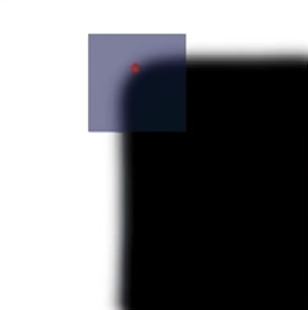
\includegraphics[width=\linewidth]{harris_on}
  \caption{Filter window on corner}\label{fig:awesome_image2}
\endminipage\hfill
\minipage{0.32\textwidth}%
  
\includegraphics[width=\linewidth]{harris_in}
  \caption{Filter window can not recognize the corner any more}\label{fig:awesome_image3}
\endminipage
\end{figure}
If the corner is scaled up and the filter window (light blue color) is on the corner’s side or on the x,y edge then we can still recognize that that is a corner, but if the filter window falls inside the corner figure, then we lose the indication of the corner.

\subsection*{RANSAC}
Random Sample Consensus, is allowing us effectively remove outliers and determine the strongest linear model of the dataset.

\begin{figure}[h]
\centering
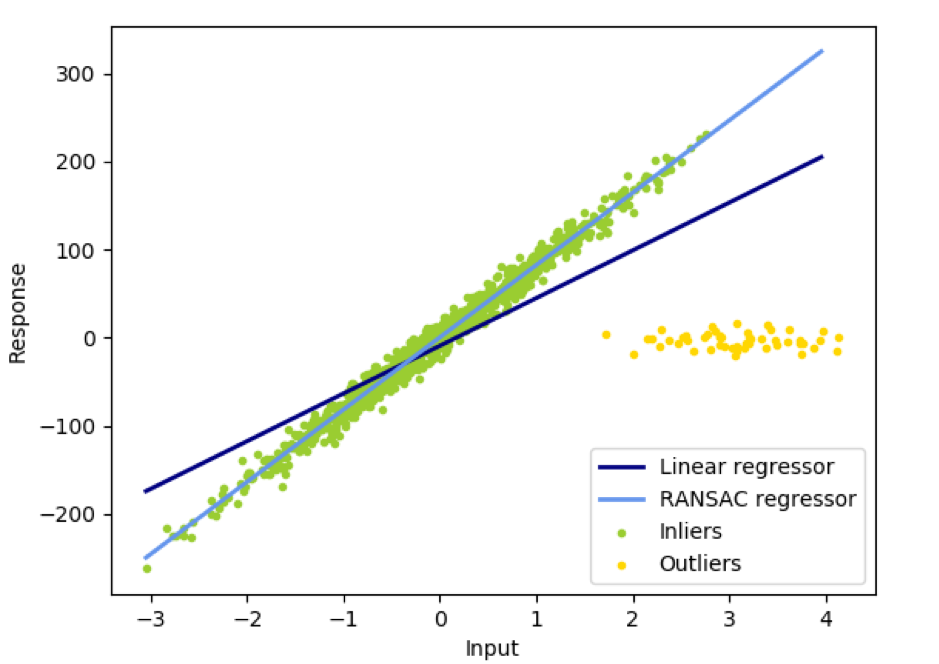
\includegraphics[width=8cm]{RANSAC}
\captionof{figure}[6.5pt]{RANSAC model vs. Linear regressor }
\end{figure}

As we can see in the example above, there is two lines (models). One for the Linear regression and one for the RANSAC. Because of the outliers (yellow dot group) the Linear model has wrong estimation, on the other hand RANSAC model show’s the most estimated model by ignoring the false data (outliers). The model runs on iteration over the dataset, on each iteration it selects randomly 4 dots, and calculate the distances from them to the line. After that the model checks how mush data is placed near (by some delta) or on that line. The model with maximum number of dataset that placed on the same line returned.
After running RANSAC we render two images that show’s the inliers and the outliers of the images.

\subsection*{Homography}
After using the RANSAC, we determine the inliers that best fit to the model. Now we want to fine the matrix that will transform one plane pixel to another plane, we want transform image2 to the plane of image1.
When an image is transformed to another image’s plane, it ensures that the epilines in both images are parallel to this image plane. This is a useful property that can be harnessed to reduce the number of searches while matching keypoints in 2 images, since a given point in an image will lie on the corresponding epiline in the other image (observed from a different point in space). 
\\
Homography can be mathematically expressed as 
\begin{gather*}
\begin{bmatrix}x' \\ y' \\ 1 \end{bmatrix}
 =
  \begin{bmatrix}
    h_1_1      & h_1_2       & h_1_3     \\
    h_2_1      & h_2_2      & h_2_3    \\
    h_3_1      & h_3_2      & h_3_3    \\
\end{bmatrix}
    \begin{bmatrix}x \\ y \\ 1 \end{bmatrix}
\end{gather*}
\newpage

\subsection*{Our Test and Results}
We implemented the RANSAC from scratch, used the OpenCV feature detection with the help of SIFT, finally found the best Homogrphy and at the end made the warping. Here is our image set, the RANSAC inliers, outliers and the final panorama result.

\subsection*{Backyard}
\begin{figure}[!htb]
\minipage{0.32\textwidth}
  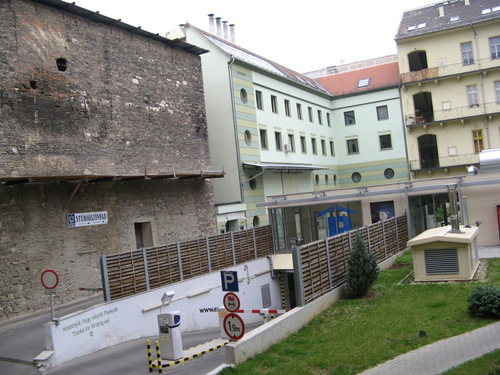
\includegraphics[width=\linewidth]{backyard1}
    \caption{backyard1}
\endminipage\hfill
\minipage{0.32\textwidth}
  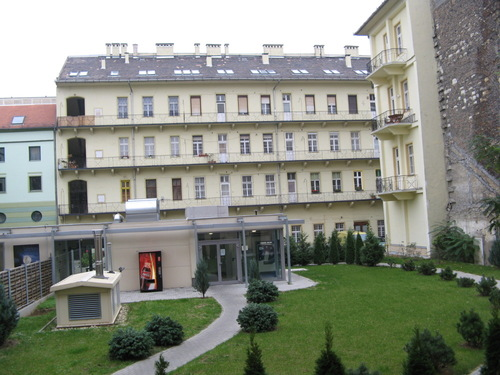
\includegraphics[width=\linewidth]{backyard2}
    \caption{backyard2}
\endminipage\hfill
\minipage{0.32\textwidth}%
  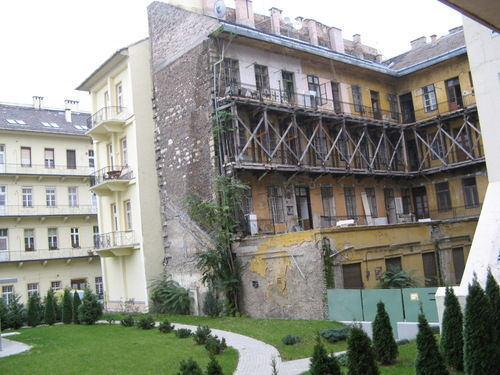
\includegraphics[width=\linewidth]{backyard3}
    \caption{backyard3}
\endminipage
\end{figure}

\begin{figure}[!htb]
\minipage{0.5\textwidth}
  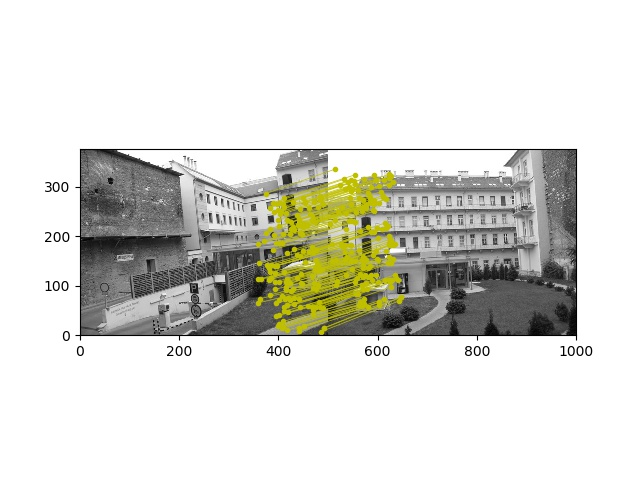
\includegraphics[width=\linewidth]{outMatches_inlier_backyard1}
      \caption{Inliers backyard1 and backyard2}
\endminipage\hfill
\minipage{0.5\textwidth}
  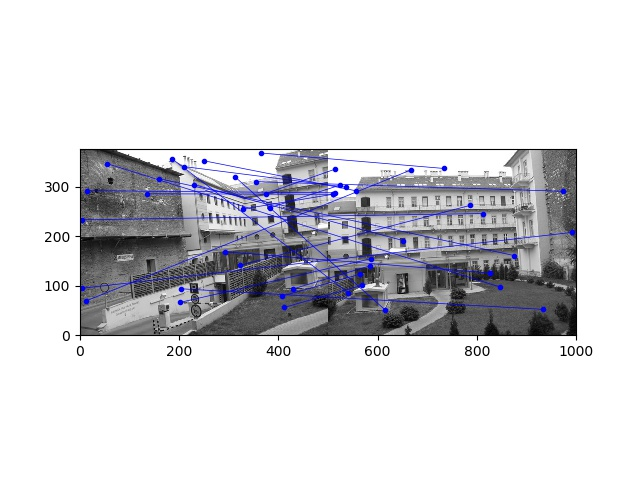
\includegraphics[width=\linewidth]{outMatches_outlier_backyard1}
      \caption{Outliers backyard1 and backyard2}
\endminipage\hfill
\end{figure}

\begin{figure}[!htb]
\minipage{0.5\textwidth}
  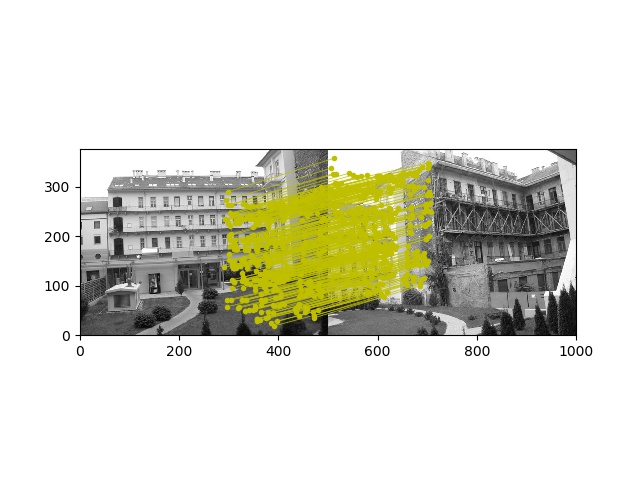
\includegraphics[width=\linewidth]{outMatches_inlier_backyard2}
        \caption{Inliers backyard2 and backyard3}
\endminipage\hfill
\minipage{0.5\textwidth}
  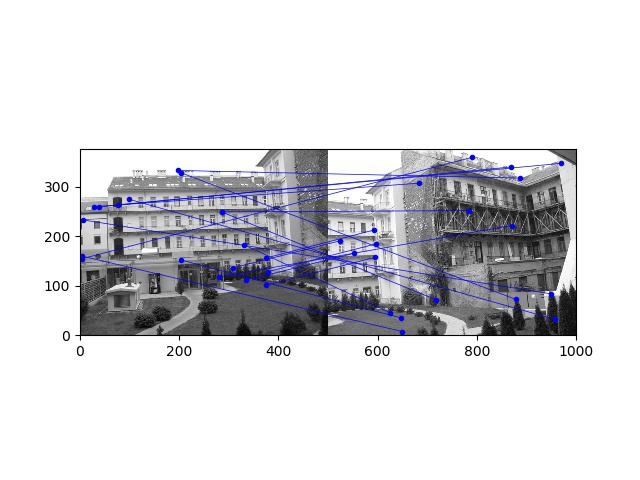
\includegraphics[width=\linewidth]{outMatches_outlier_backyard2}
        \caption{Outliers backyard2 and backyard3}
\endminipage\hfill
\end{figure}
\newpage

\subsection*{Office}
\begin{figure}[!htb]
\minipage{0.24\textwidth}
  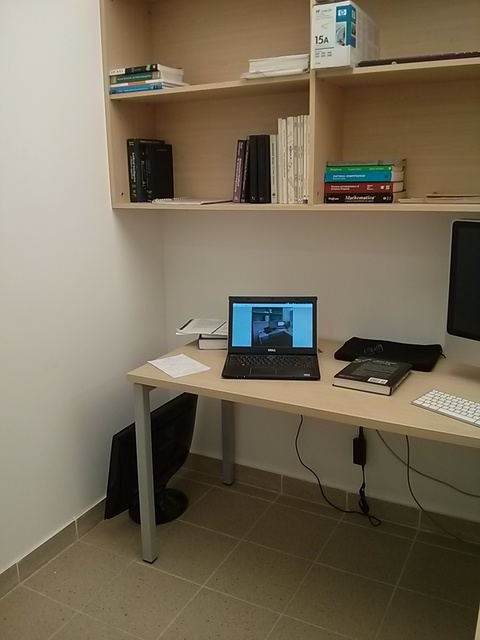
\includegraphics[width=\linewidth]{office1}
    \caption{office-1}
\endminipage\hfill
\minipage{0.24\textwidth}
  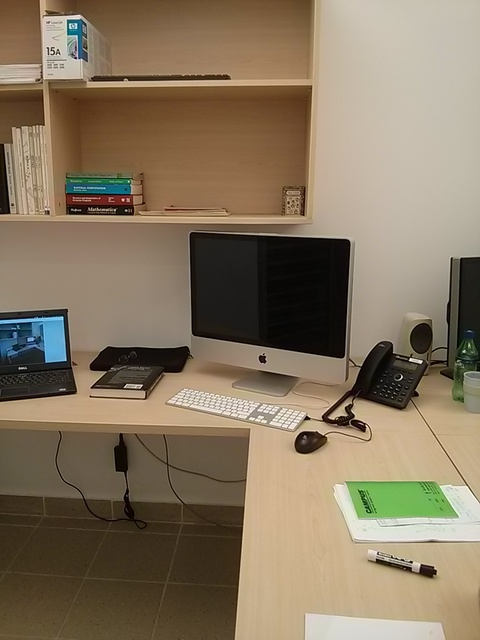
\includegraphics[width=\linewidth]{office2}
    \caption{office-2}
\endminipage\hfill
\minipage{0.24\textwidth}
  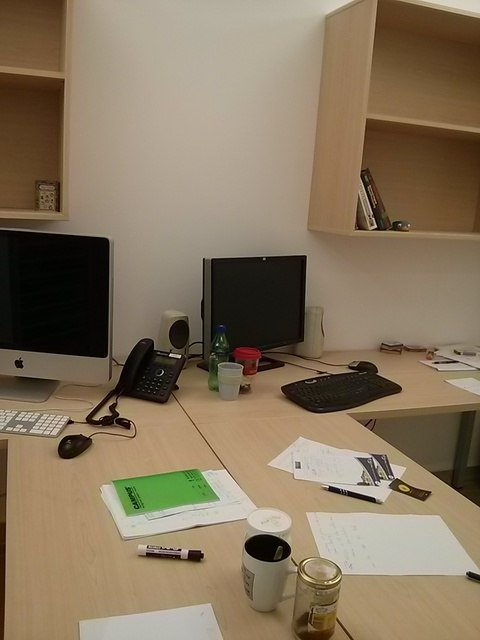
\includegraphics[width=\linewidth]{office3}
    \caption{office-3}
\endminipage\hfill
\minipage{0.24\textwidth}
  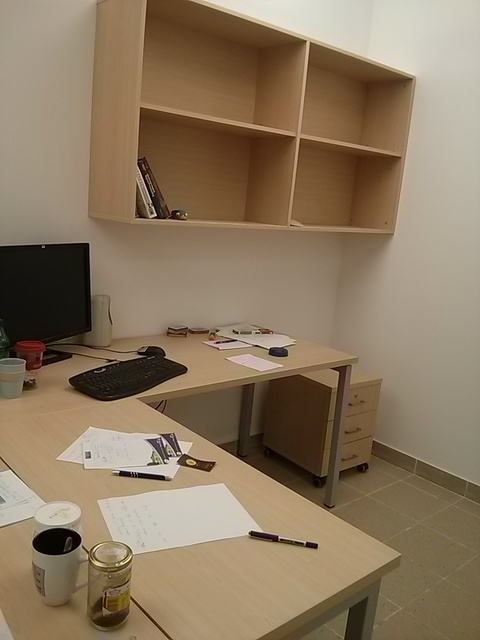
\includegraphics[width=\linewidth]{office4}
    \caption{office-4}
\endminipage\hfill
\end{figure}

\begin{figure}[!htb]
\minipage{0.5\textwidth}
  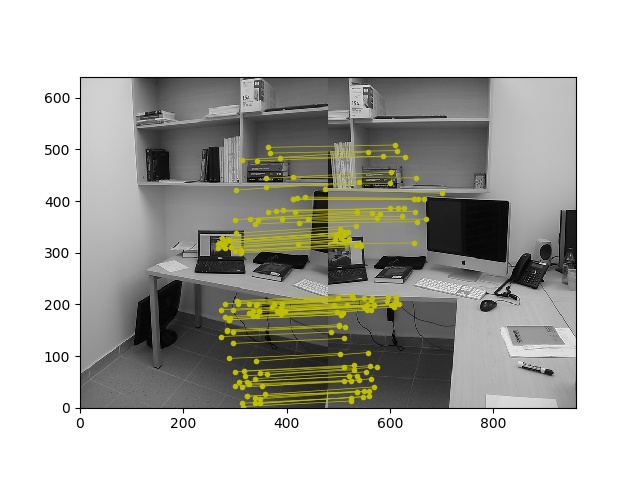
\includegraphics[width=\linewidth]{outMatches_inlier_office1}
        \caption{Inliers office1 and office2}
\endminipage\hfill
\minipage{0.5\textwidth}
  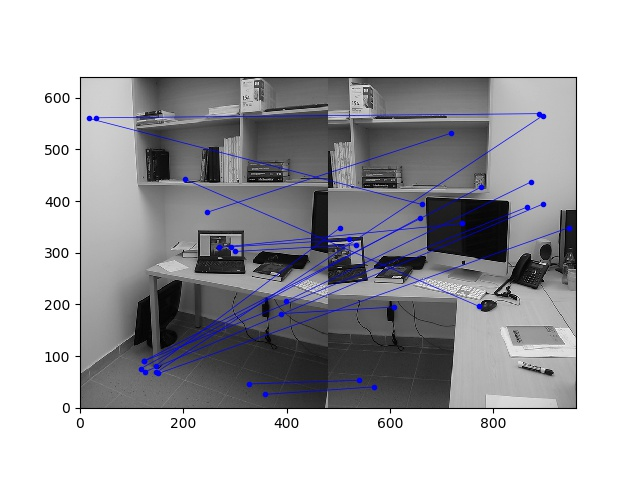
\includegraphics[width=\linewidth]{outMatches_outlier_office1}
        \caption{Outliers office1 and office2}
\endminipage\hfill
\end{figure}

\begin{figure}[!htb]
\minipage{0.5\textwidth}
  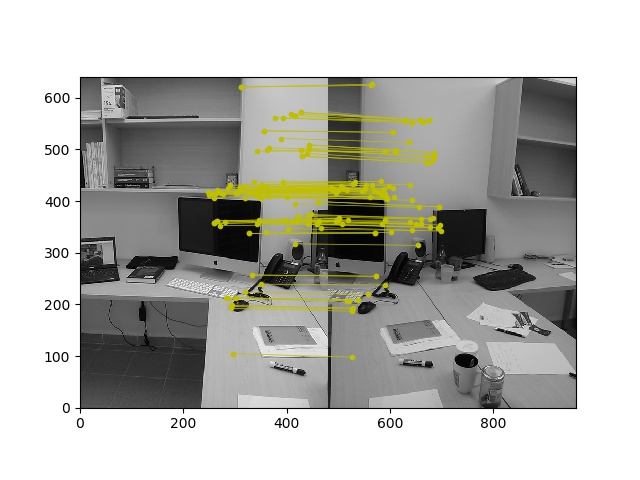
\includegraphics[width=\linewidth]{outMatches_inlier_office2}
        \caption{Inliers office2 and office3}
\endminipage\hfill
\minipage{0.5\textwidth}
  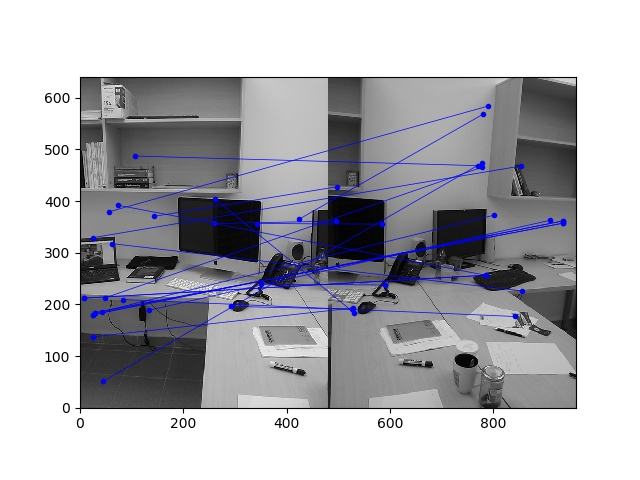
\includegraphics[width=\linewidth]{outMatches_outlier_office2}
        \caption{Outliers office2 and office3}
\endminipage\hfill
\end{figure}

\begin{figure}[!htb]
\minipage{0.5\textwidth}
  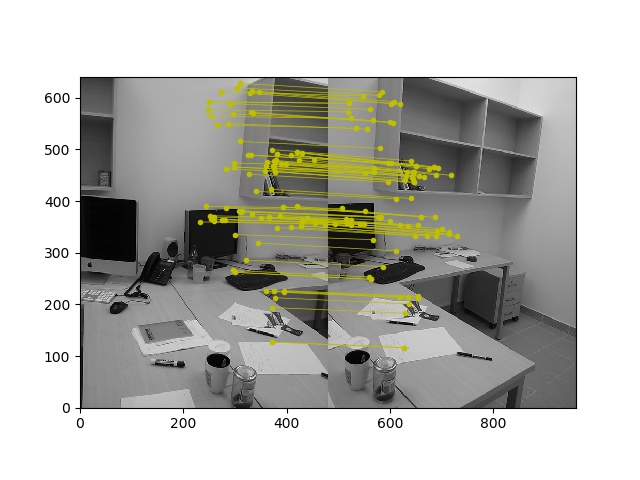
\includegraphics[width=\linewidth]{outMatches_inlier_office3}
        \caption{Inliers office3 and office4}
\endminipage\hfill
\minipage{0.5\textwidth}
  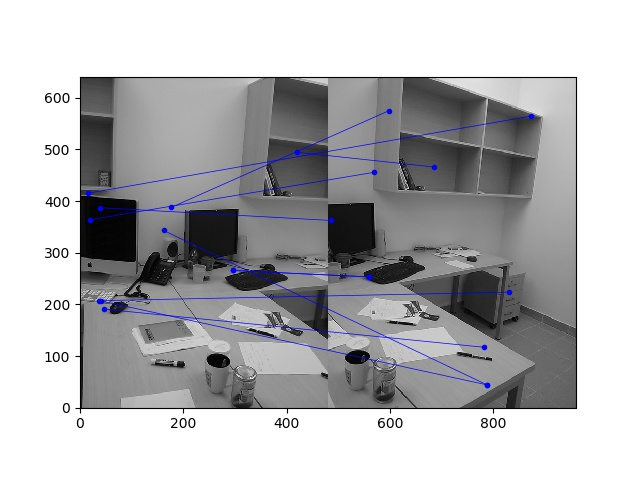
\includegraphics[width=\linewidth]{outMatches_outlier_office3}
        \caption{Outliers office3 and office4}
\endminipage\hfill
\end{figure}

\newpage
\subsection*{Panorama}
\begin{figure}[!htb]
\centering
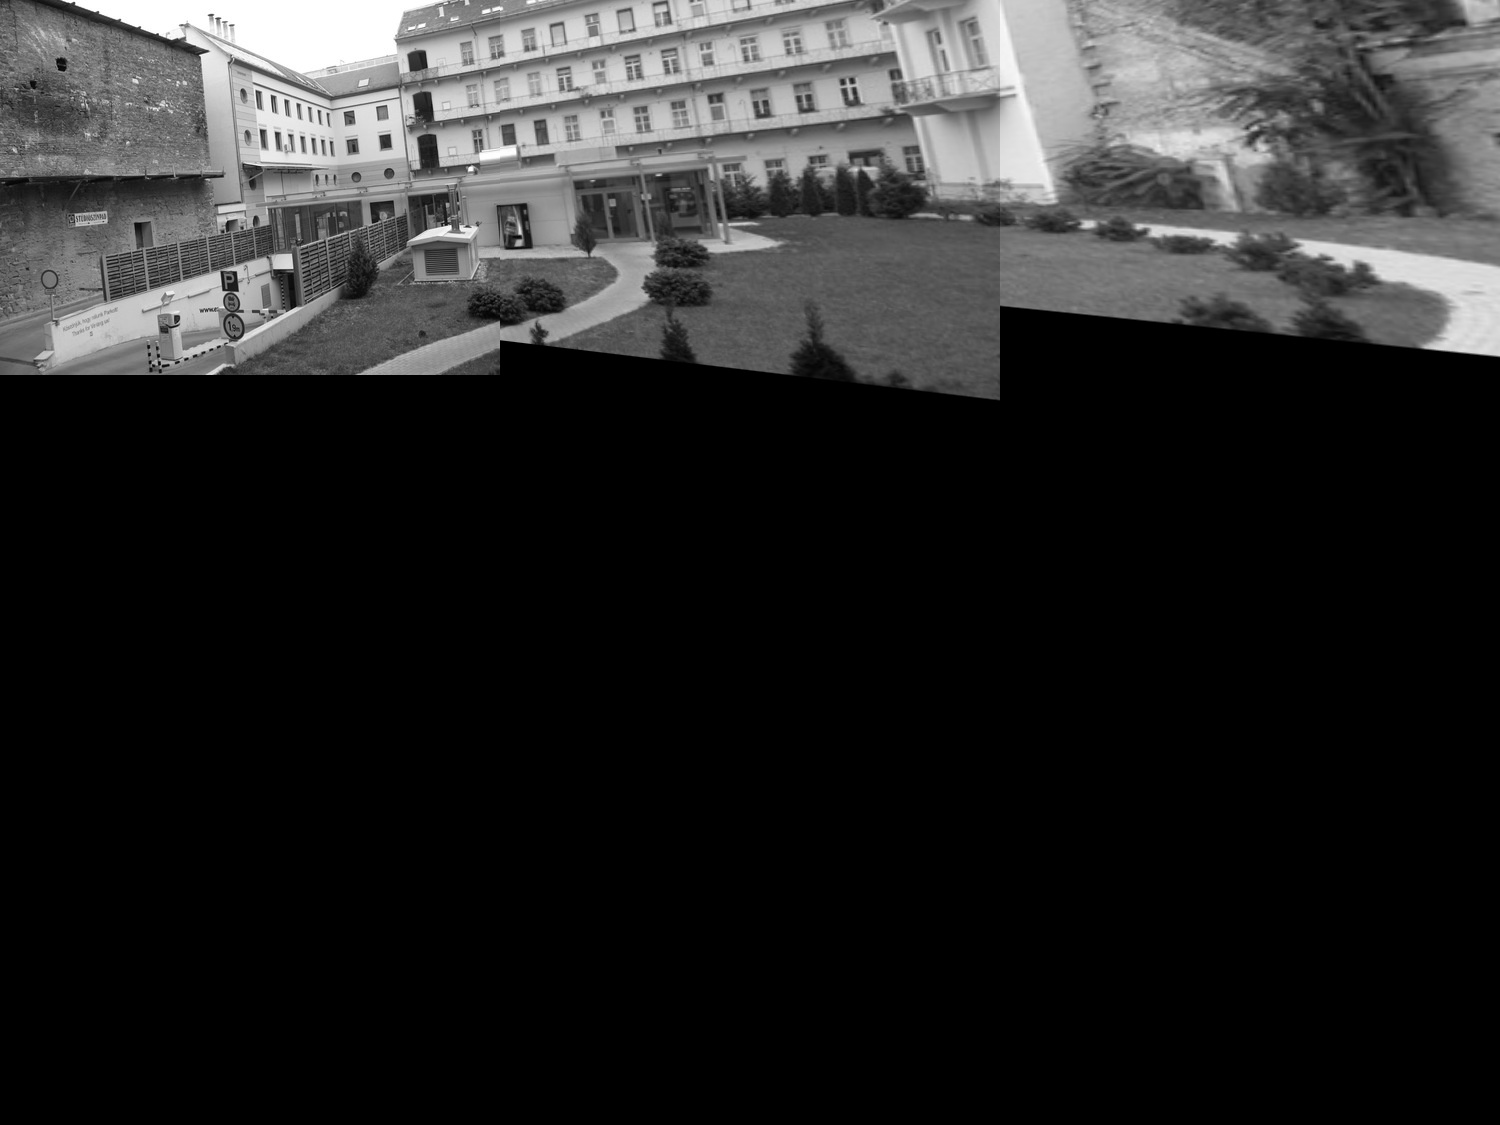
\includegraphics[width=8cm]{panorama1}
\captionof{figure}[6.5pt]{Panorama Backyard}
\end{figure}

\begin{figure}[!htb]
\centering
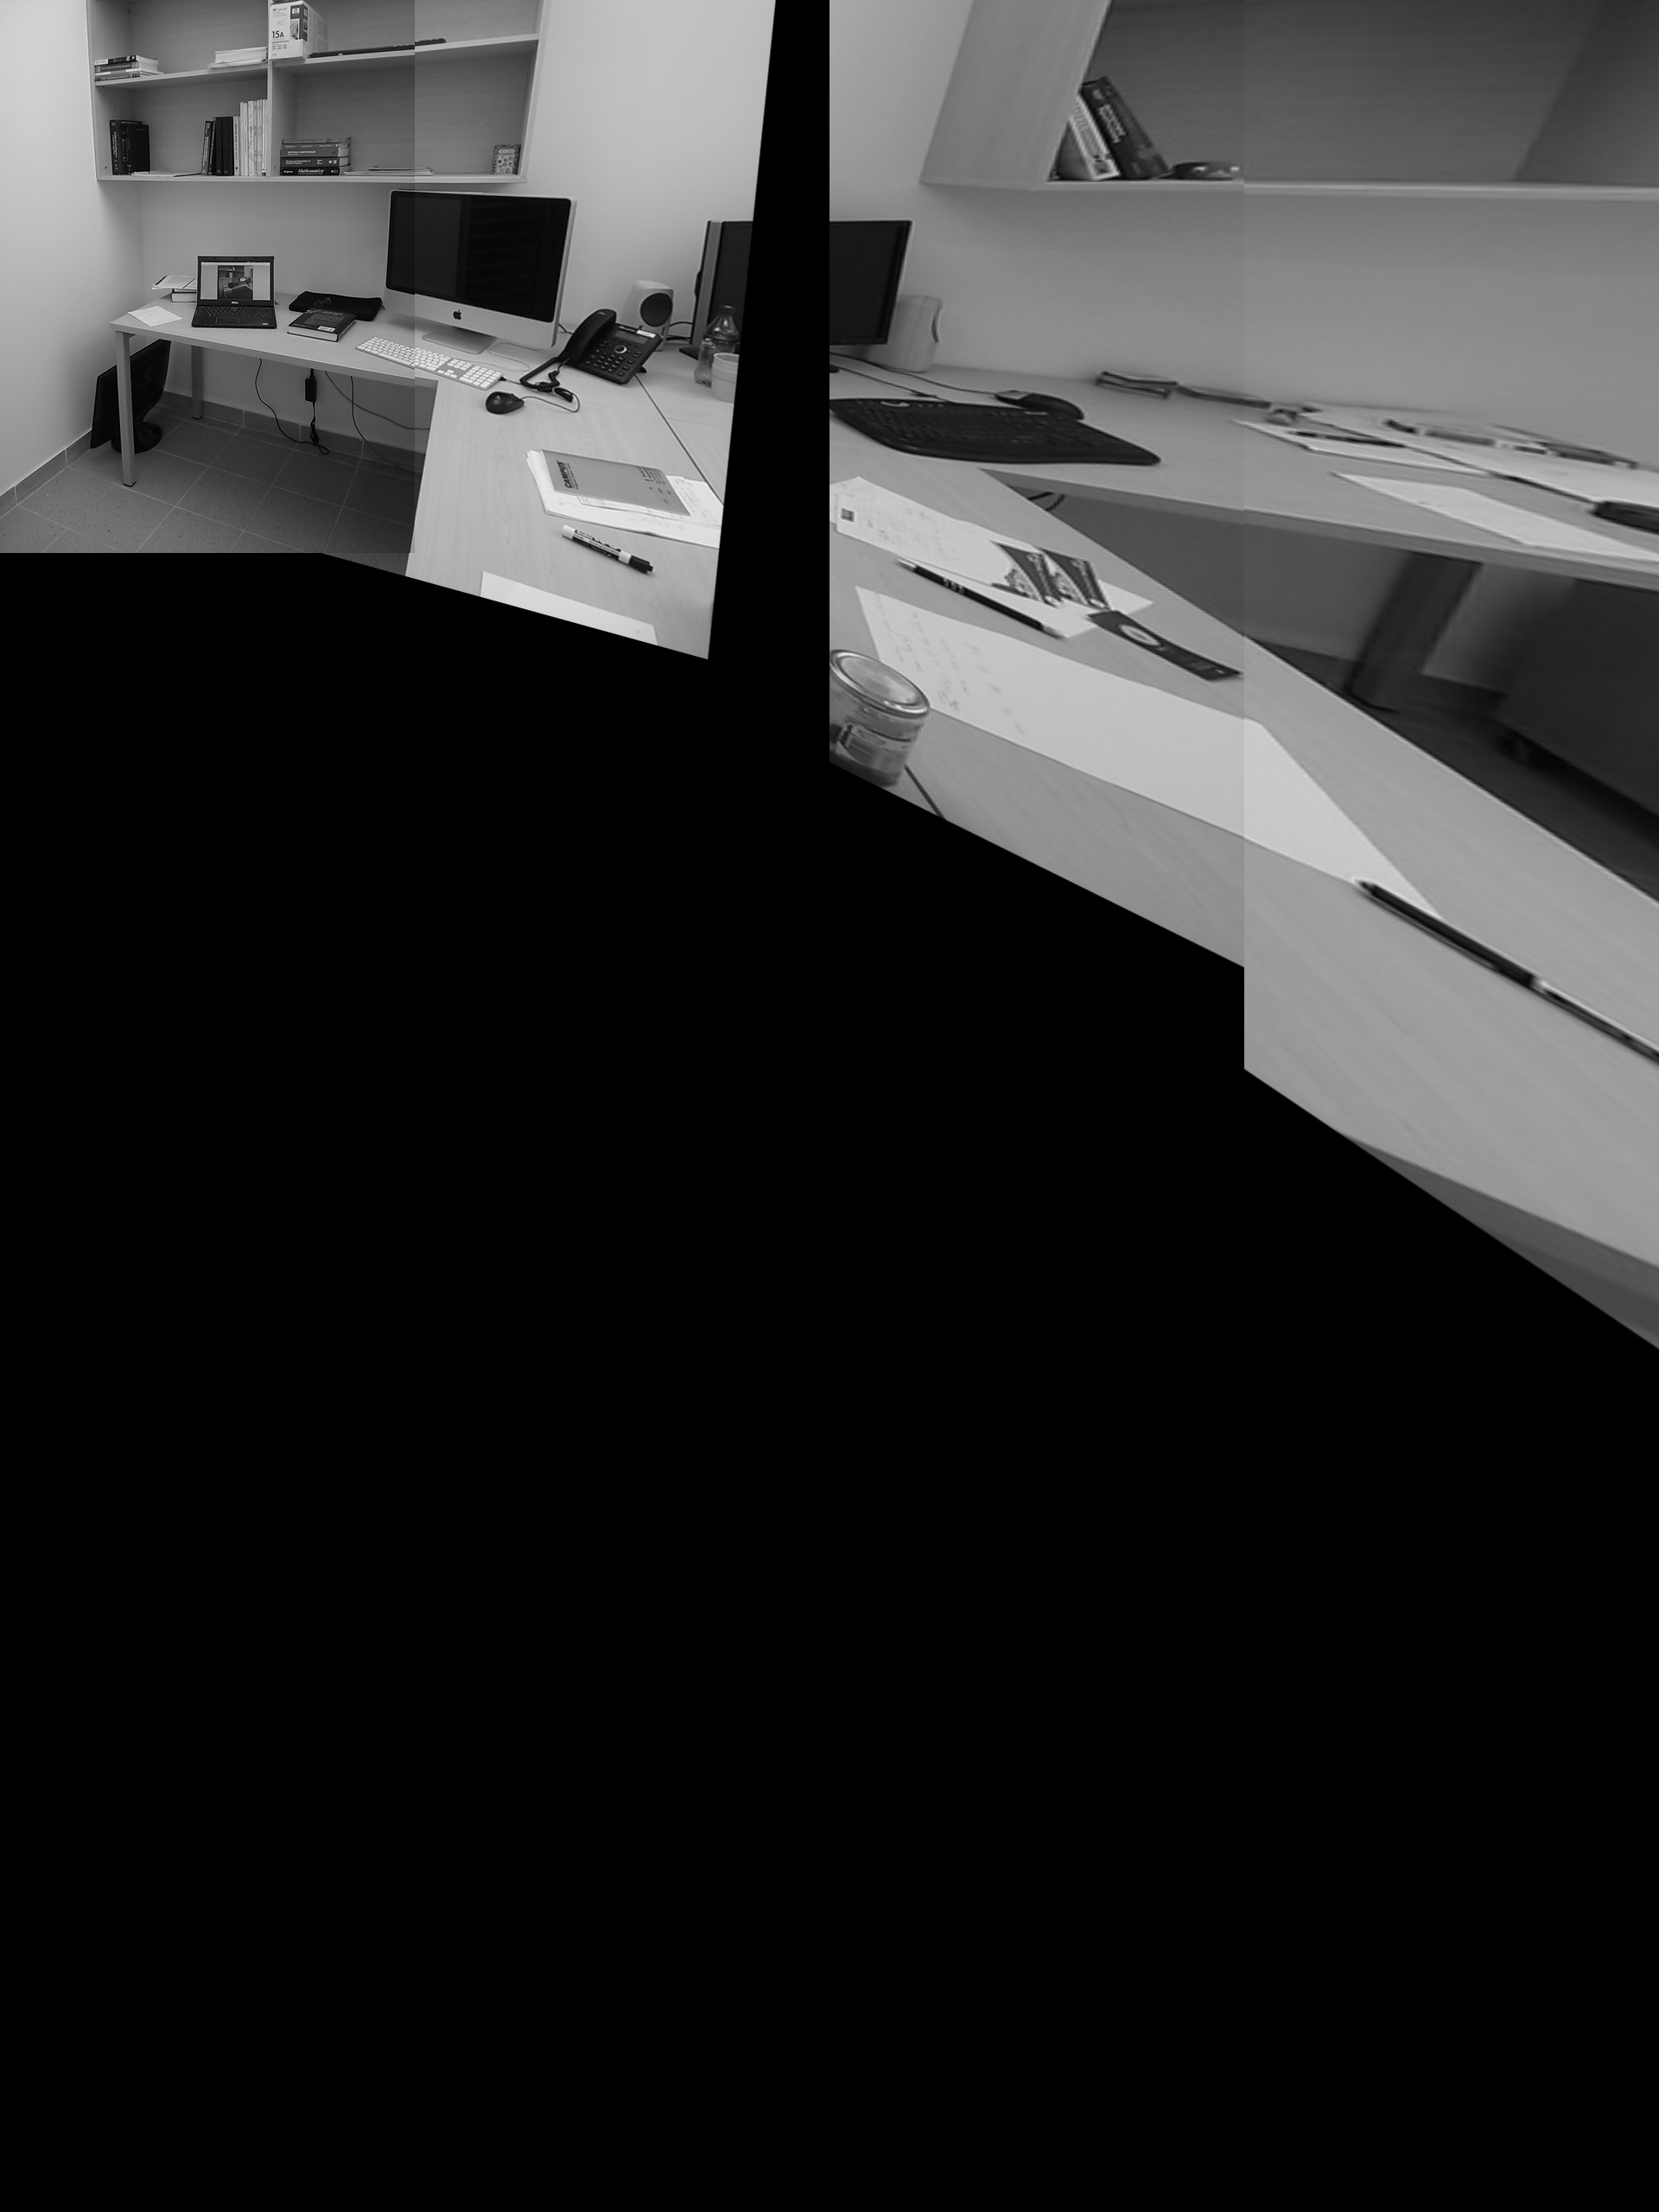
\includegraphics[width=8cm]{panorama2}
\captionof{figure}[6.5pt]{Panorama Office}
\end{figure}




















\end{document}